\documentclass[a4paper, 12pt, english]{article}

% \usepackage[portuges]{babel}
\usepackage[utf8]{inputenc}
\usepackage{amsmath,amssymb}
\usepackage{graphicx}
\usepackage{subfig}
\usepackage[colorinlistoftodos]{todonotes}

\usepackage{indentfirst}
\usepackage{verbatim}
\usepackage{textcomp}
\usepackage{gensymb}
\usepackage{float}

\usepackage{relsize}

\usepackage{lipsum}% http://ctan.org/pkg/lipsum
\usepackage{xcolor}% http://ctan.org/pkg/xcolor
\usepackage{xparse}% http://ctan.org/pkg/xparse
\NewDocumentCommand{\myrule}{O{1pt} O{2pt} O{black}}{%
	\par\nobreak % don't break a page here
	\kern\the\prevdepth % don't take into account the depth of the preceding line
	\kern#2 % space before the rule
	{\color{#3}\hrule height #1 width\hsize} % the rule
	\kern#2 % space after the rule
	\nointerlineskip % no additional space after the rule
}
\usepackage[section]{placeins}

\usepackage{booktabs}
\usepackage{colortbl}%
\newcommand{\myrowcolour}{\rowcolor[gray]{0.925}}

\usepackage[obeyspaces]{url}
\usepackage{etoolbox}
\usepackage[colorlinks,citecolor=black,urlcolor=blue,bookmarks=false,hypertexnames=true]{hyperref}

\usepackage{geometry}
\geometry{
	paper=a4paper, % Change to letterpaper for US letter
	inner=3cm, % Inner margin
	outer=3cm, % Outer margin
	bindingoffset=.5cm, % Binding offset
	top=2cm, % Top margin
	bottom=2cm, % Bottom margin
	%showframe, % Uncomment to show how the type block is set on the page
}
\usepackage{fancyhdr}

% Define header and footer
\pagestyle{fancy}
\fancyhf{}
\lhead{ENER 104L}
\rhead{iSciM, Habib University} % Right-aligned page number in the header
\rfoot{\thepage} % Right footer text
%*******************************************************************************%
%************************************START**************************************%
%*******************************************************************************%
\begin{document}

%************************************TITLE PAGE**************************************%
\begin{titlepage}
	\begin{center}
		\textbf{\LARGE Habib University}\\[0.5cm]
		\textbf{\large iSciM}\\[0.2cm]
		\textbf {\large Fall 2023}\\[0.2cm]
		\vspace{20pt}
		
\includegraphics[width=5cm]{../habiblogo.jpg}\\[1cm]
		\par
		\vspace{20pt}
		\textbf{\Large ENER 104L RENEWABLE ENERGY}\\
		\vspace{15pt}
		\myrule[1pt][7pt]
		\textbf{\LARGE  LABORATORY REPORT 12}\\
		\vspace{15pt}
		\textbf{\large Bioplastic}\\
		\myrule[1pt][7pt]
		\vspace{25pt}
		\begin{tabular}{@{}p{5cm}p{3cm}@{}}
			\textbf{\large Student Name} & \textbf{\large Student ID} \\
			Ali Asghar Yousuf            & ay06993                    \\ % No1 
			Syed Ibrahim Ali Haider      & sh06565                    \\ % No2
		\end{tabular}

		\vspace{10pt}
		\begin{tabular}{@{}p{5cm}p{3cm}@{}}
			\textbf{\large Group Name} & \textbf{\large Group No.} \\
			Insane Fr                  & 1                         \\
		\end{tabular}

		\vspace{45pt}
		\textbf {\large Lab Instructors:}\\[0.2cm]
		\Large {Paishwa Naqvi}\\[0.1cm]
		\Large {Mah Noor Jamil}\\[0.1cm]
		\Large {Amber Talat}\\[0.1cm]
	\end{center}

	\par
	\vfill
	\begin{center}
		\textbf{\today}\\
	\end{center}

\end{titlepage}

%************************************TABLE OF CONTENTS**************************************%

%  %Sumário
%  \newpage
%  \tableofcontents
%  \thispagestyle{empty}
%  %End Sumário

%********************************%
%***********SECTION 1************%
%********************************%
\newpage
\section{Objectives}
\begin{itemize}
	\item To create a bioplastic from potato starch.
	\item To understand the role of plasticizer in the formation of bioplastic.
\end{itemize}

\section{Abstract}
Plastics are a major part of our lives. They are used in almost every aspect of
our lives. However, the plastic that we use is not biodegradable and is harmful
to the environment. Bioplastics are a solution to this problem. They are
biodegradable and are made from renewable resources. In this experiment, we
will be making bioplastic from potato starch using glycerol as a plasticizer
and acetic acid to break down the amylopectin in the potato starch. We made two
samples of bioplastic, one with glycerol and one without glycerol.

\section{Result and Analysis}
\subsection{Sample 1}
We made the first sample of bioplastic with glycerol.

\begin{figure}[H]
	\centering
	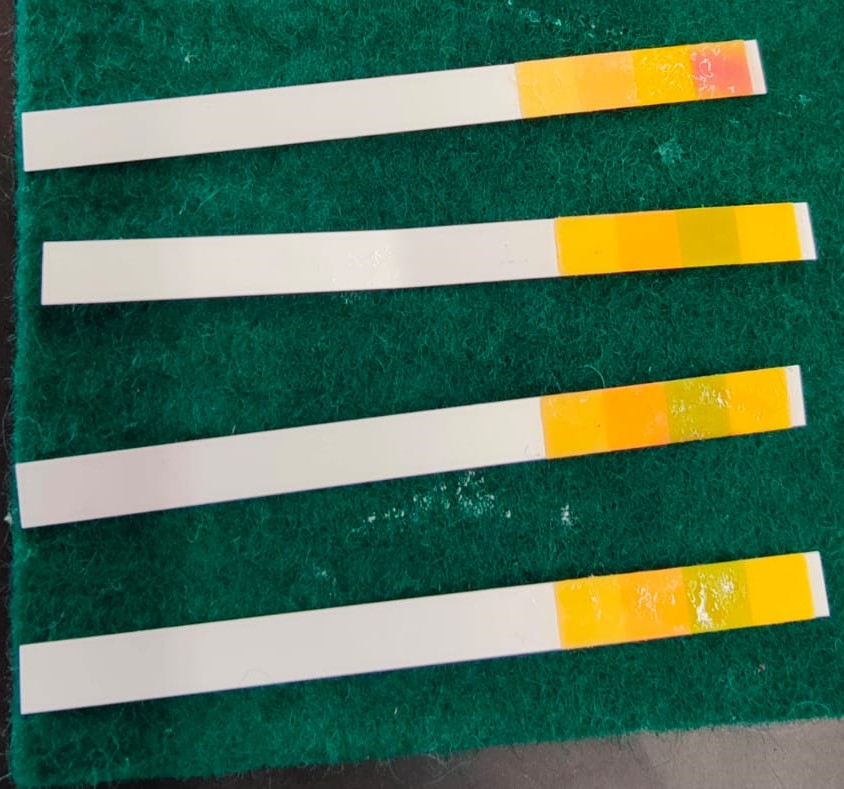
\includegraphics[width=0.5\textwidth]{images/sample1-ph.jpg}
	\caption{Sample 1 PH}
	\label{fig:sample1-ph}
\end{figure}

Initially the PH of our mixture was around 3 due to the presence of acetic acid
in the mixture. We gradually added sodium hydroxide solution to the mixture to
neutralize the acetic acid, which is an important step in the formation of
bioplastic. If the acetic acid is not neutralized, the bioplastic will not form
properly and will not be able to hold its shape.

We let the mixture dry for a few days and then removed the bioplastic from the
mould. The bioplastic was very goeey and sticky. It had not dried properly and
was not able to hold its shape.

\begin{figure}[H]
	\centering
	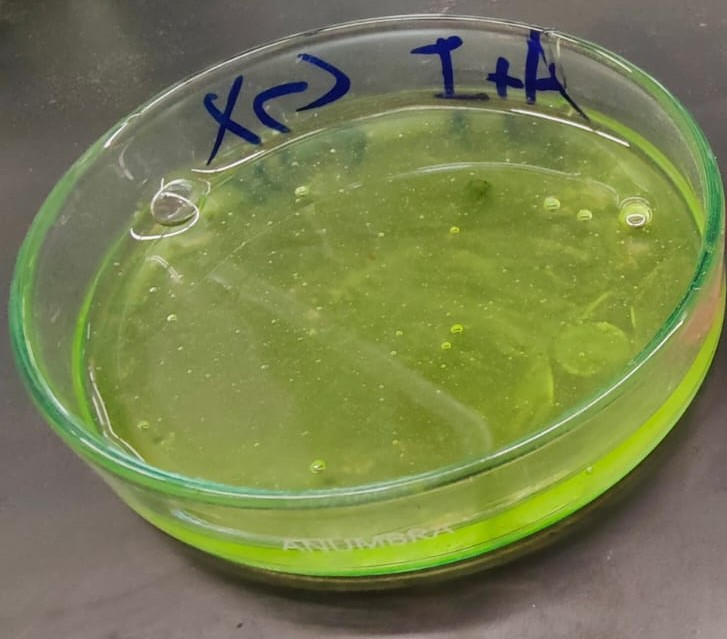
\includegraphics[width=0.5\textwidth]{images/sample1.jpg}
	\caption{Sample 1}
	\label{fig:sample1}
\end{figure}
\subsection{Sample 2}
We made the second sample of bioplastic without glycerol.

\begin{figure}[H]
	\centering
	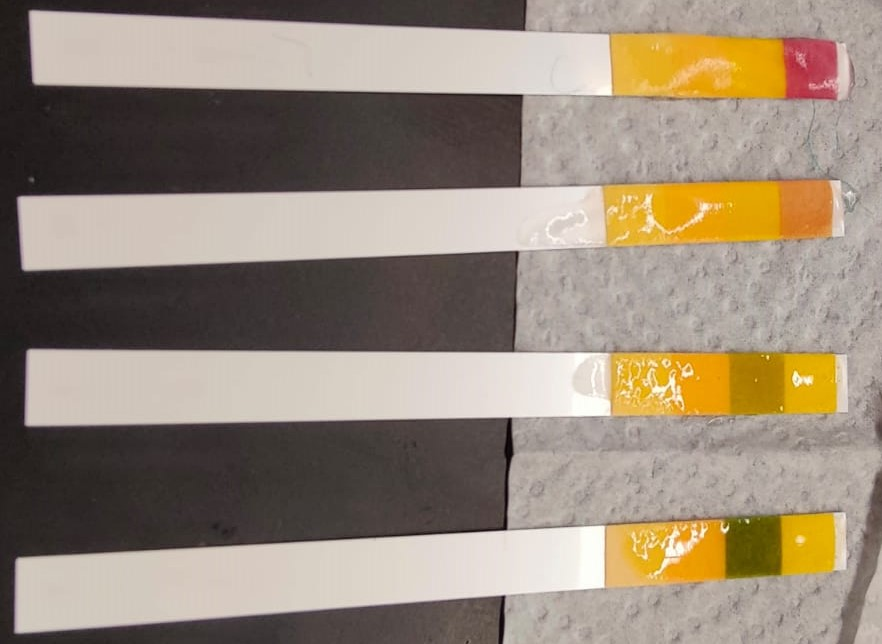
\includegraphics[width=0.5\textwidth]{images/sample2-ph.jpg}
	\caption{Sample 2 PH}
	\label{fig:sample2-ph}
\end{figure}

We followed the same procedure as sample 1. We let the mixture dry for a few
days and then tried to remove the bioplastic from the mould but it was not
possible. The bioplastic had dried and was not sticky anymore but it was very
hard and brittle. It was not able to hold its shape and broke into pieces when
we tried to remove it from the mould.

\begin{figure}[H]
	\centering
	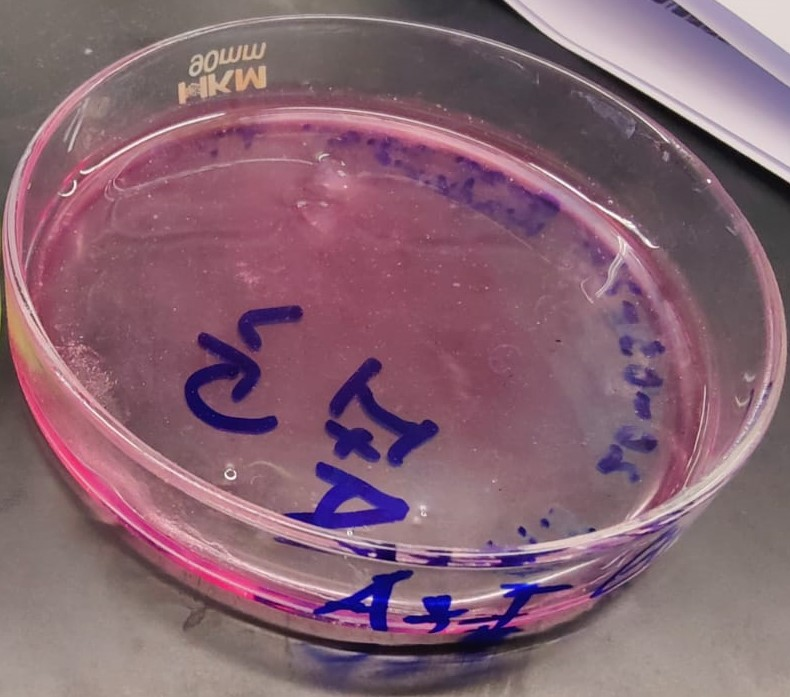
\includegraphics[width=0.5\textwidth]{images/sample2.jpg}
	\caption{Sample 2}
	\label{fig:sample2}
\end{figure}

\subsection{Analysis}
We were not able to make a proper bioplastic. The bioplastic we made was either
too sticky or too brittle. We were not able to find the right balance between
the two. We think that the reason for this is that we did not add the right
amount of glycerol. We added too much glycerol in the first sample and none in
the second sample. We think that if we had added the right amount of glycerol,
we would have been able to make a proper bioplastic.

\section{Conclusion}
Despite our results not being ideal, we were able to learn a lot from this
experiment. We learned that the amount of glycerol is very important in the
formation of bioplastic and the role of acid in the formation of bioplastic.

Bioplastics are a great alternative to conventional plastics. They are
biodegradable and are made from renewable resources. They are not harmful to
the environment. They are also very cheap and easy to make. They can be used in
a variety of applications such as packaging, food containers, and many more.
This step towards a more sustainable future is very important and we should
continue to research and develop bioplastics.

\section{Questions}
\begin{enumerate}
	\item What difference has adding the propan-1,2,3-triol made?

	      \textbf{Answer:} The propan-1,2,3-triol acts as a plasticizer. It makes the
	      bioplastic more flexible and less brittle.

	\item Why is acetic acid used?

	      \textbf{Answer:} Acetic acid is used to break down the amylopectin in the
	      potato starch. Amylopectin is a branched polymer of glucose. It is a
	      polysaccharide. It is a major component of starch.

	\item Do you think the plastic you made from potato starch will be biodegradable?
	      Explain your answer?

	      \textbf{Answer:} Yes, the plastic we made from potato starch will be
	      biodegradable. It is made from potato starch which is a renewable resource.
	      It is also made from glycerol which is a natural compound. It is also
	      biodegradable. The plastic we made is also biodegradable because it is made
	      from natural compounds and is not harmful to the environment.

	\item Explain the meaning of the terms bioplastic and biodegradable.

	      \textbf{Answer:} Bioplastic is a type of plastic that is made from renewable
	      resources. It is also biodegradable. Biodegradable means that it can be
	      broken down by microorganisms and other living organisms. It is not harmful to
	      the environment.

	\item Write a list of the advantages of making plastics for which the raw material
	      comes from plants.

	      \textbf{Answer:} The advantages of making plastics from plants are:
	      \begin{itemize}
		      \item The raw material is renewable.
		      \item The raw material is biodegradable.
		      \item The raw material is not harmful to the environment.
		      \item The raw material is cheap and easily available.
	      \end{itemize}

	\item What are the disadvantages? (Hint: think about growing the plants).

	      \textbf{Answer:} The disadvantages of making plastics from plants include the requirement of large amounts of space, water, and nutrients for plant cultivation. Additionally, the growth process of plants is time-consuming. These factors contribute to the overall cost and resource-intensive nature of plant-based plastic production.
\end{enumerate}

\end{document}